
\section{Deliverable 6: Non-linear embeddings}


\subsection{Circular Data, Non-Linear Embedding: $x^2 + y^2$}

\begin{solve}    
\begin{lstlisting}[language=python, title = MLP used for linearly separable data after adding non linear feature]
dim_in, dim_out = 3, 2
hidden_neuron_list = [1]
activation_list = ['ReLU', 'Sigmoid']
opt_init = 'xavier'
opt_loss = L2Loss()
mlp = MLP(dim_in, dim_out, hidden_neuron_list, activation_list, opt_init)
opt_optim = Adam(mlp)
print(mlp.summary())
    
-----------------------------------------------------------------
Model Summary
-------------
Layer 1: Linear - A Dim: 3, Output Dim: 1, Parameters: 4
Layer 2: ReLU
Layer 3: Linear - A Dim: 1, Output Dim: 2, Parameters: 4
Layer 4: Sigmoid
Total Parameters: 8
\end{lstlisting}
    
\begin{figure}
    \centering
    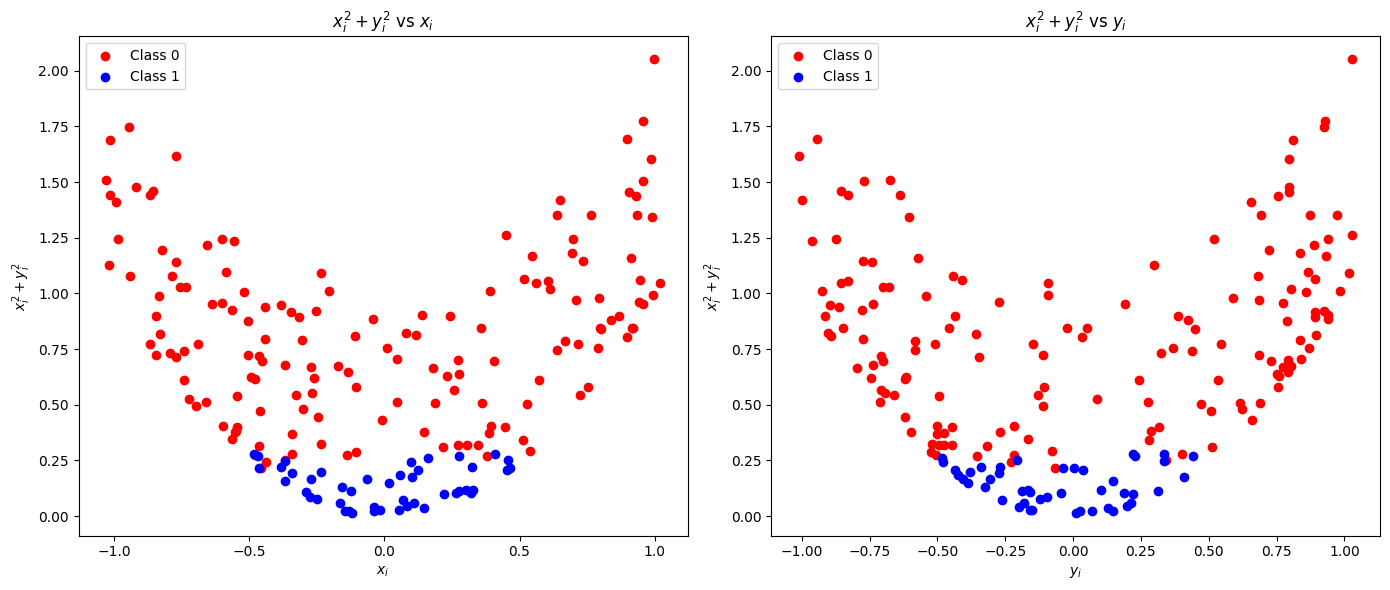
\includegraphics[width=0.7\textwidth]{plots/7_circle_transformation.png}
    \caption{Circular dataset (train, test set with 200 points each) after non-linear embedding}
\end{figure}


\begin{figure}[H]
    \centering
    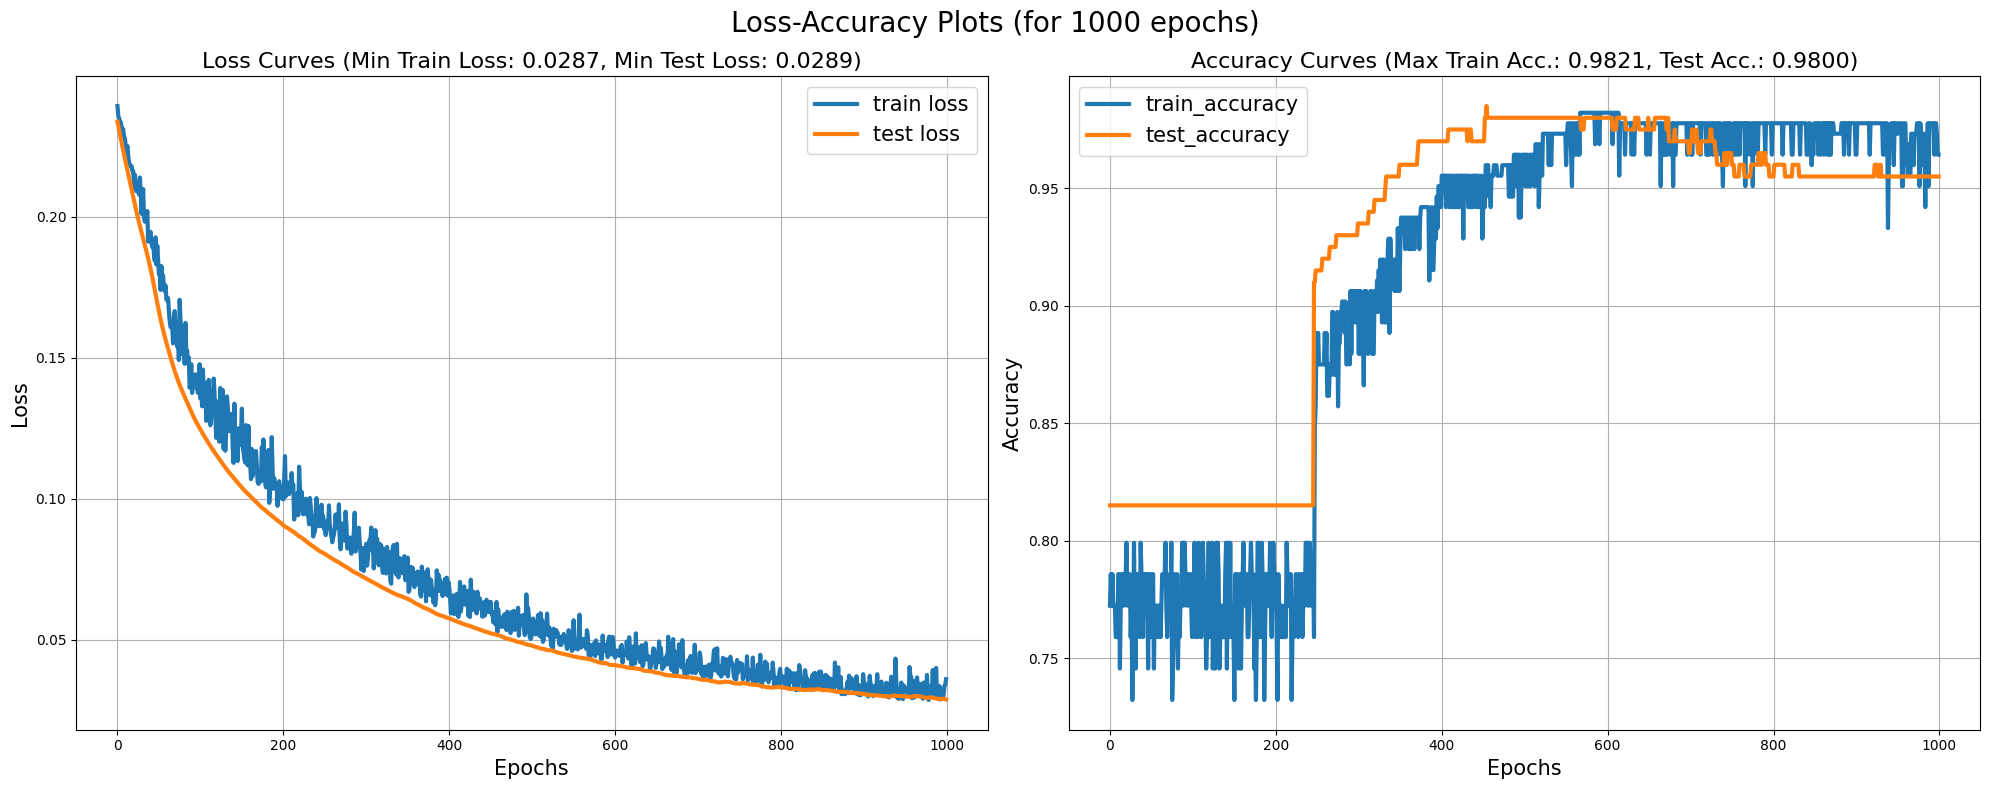
\includegraphics[width=0.8\textwidth]{plots/7_circle_loss_acc.png}
    \caption{Loss Accuracy plot for circular data after adding $x^2 + y^2$ feature, with MLP of 1 hidden neuron}

    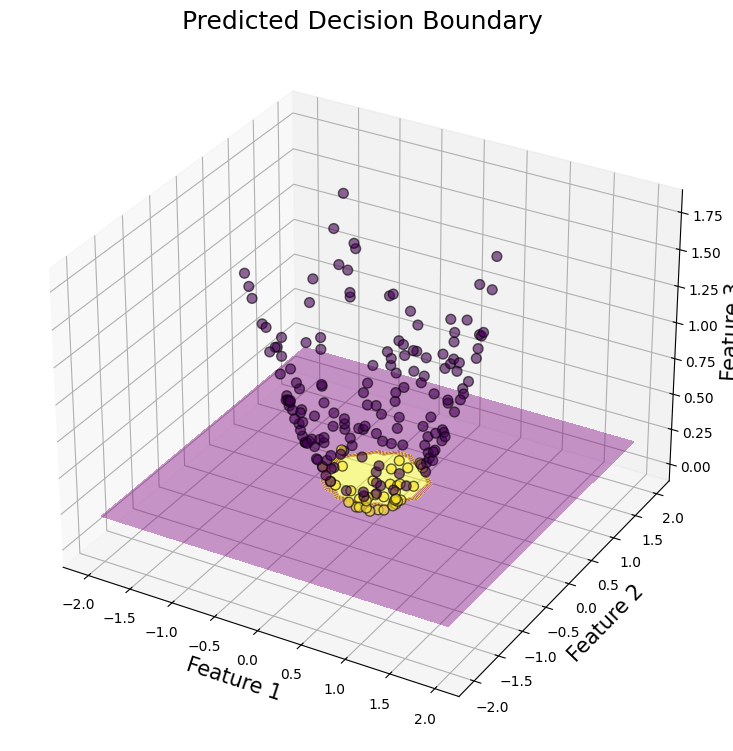
\includegraphics[width=0.7\textwidth]{plots/7_circle_db.png}
    \caption{Predicted Decision boundary for circular data after adding $x^2 + y^2$ feature (x: feature 1, y: feature 2, $x^2 + y^2$: feature 3). We see that the decision boundary after adding the non-linear feature is a hyperplane across the purple and yellow points.}
\end{figure}

\end{solve}
%%%%% ############################################


\subsection{XOR Data, Non-Linear Embedding: $x\times y$}

\begin{solve} 
Same model as above (that was used for circular data) is used for XOR data after adding non-linear feature $x\times y$.


\begin{figure}
    \centering
    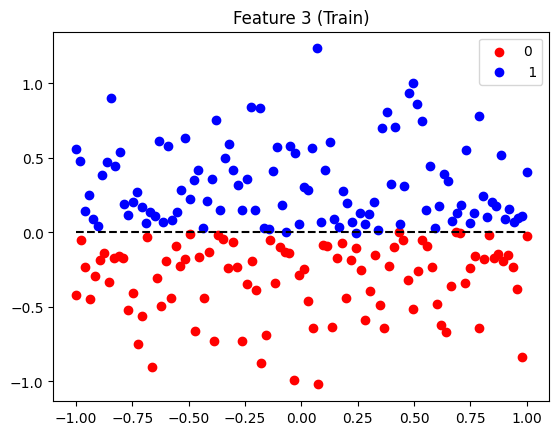
\includegraphics[width=0.7\textwidth]{plots/7_xor_transformation.png}
    \caption{XOR dataset (train, test set with 200 points each) after non-linear embedding (x: feature 1, y: feature 2, $x\times y$: feature 3)}
\end{figure}


\begin{figure}[H]
    \centering
    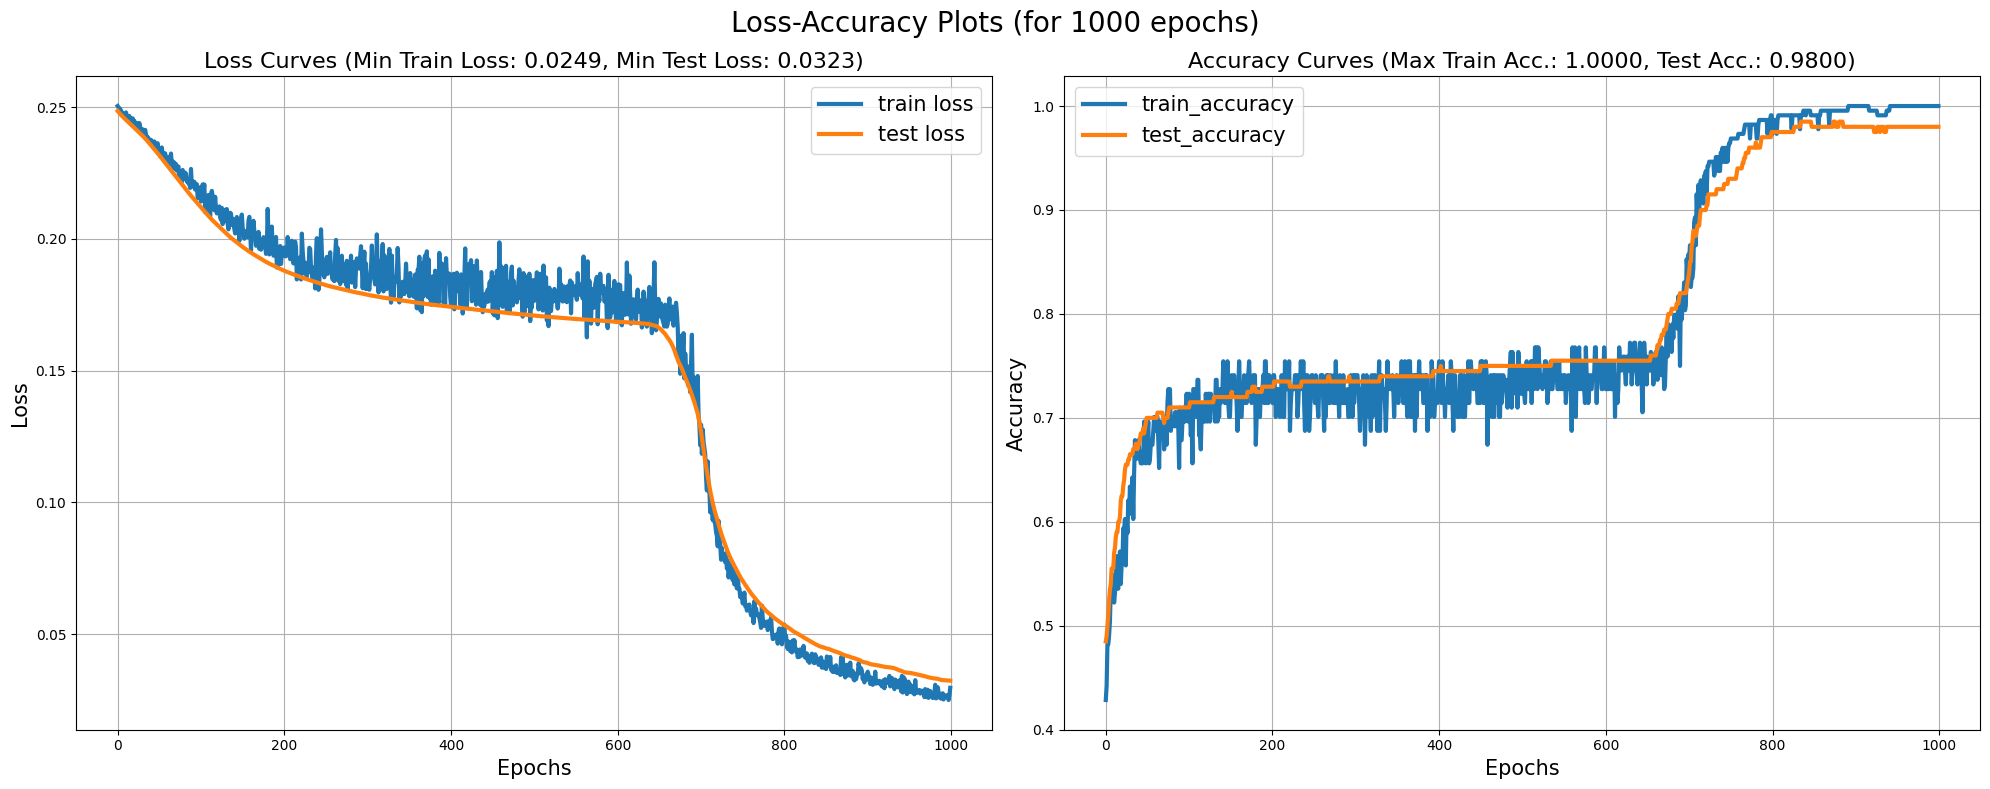
\includegraphics[width=0.8\textwidth]{plots/7_xor_loss_acc.png}
    \caption{Loss Accuracy plot for circular data after adding $x^2 + y^2$ feature, with MLP of 1 hidden neuron}

    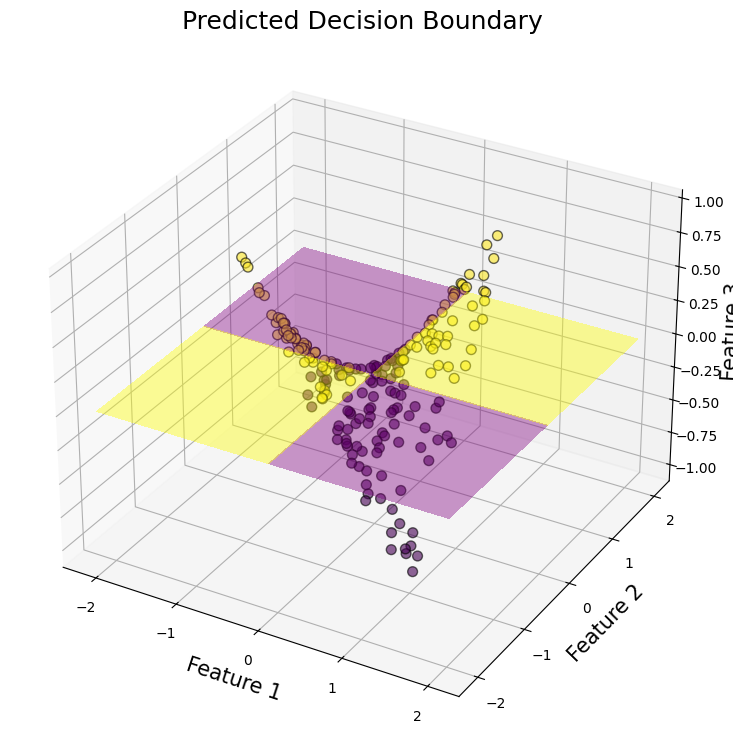
\includegraphics[width=0.7\textwidth]{plots/7_xor_db.png}
    \caption{Predicted Decision boundary for xor data after adding $x\times y$ feature (x: feature 1, y: feature 2, $x\times y$: feature 3)}
\end{figure}

\end{solve}
% ############################################

\subsection{Swiss-Roll Data, Non-Linear Embedding: $x^2, x\times y, y^2$}


\begin{solve}    
\begin{lstlisting}[language=python, title = MLP used for swiss-roll data after adding non linear features]
dim_in, dim_out = 5, 2
hidden_neuron_list = [8,4]
activation_list = ['ReLU','ReLU','Tanh']
opt_init = 'xavier'
opt_loss = L2Loss()
mlp = MLP(dim_in, dim_out, hidden_neuron_list, activation_list, opt_init)
opt_optim = Adam(mlp, learning_rate=.001)
print(mlp.summary())

-----------------------------------------------------------------
Model Summary
-------------
Layer 1: Linear - A Dim: 5, Output Dim: 8, Parameters: 48
Layer 2: ReLU
Layer 3: Linear - A Dim: 8, Output Dim: 4, Parameters: 36
Layer 4: ReLU
Layer 5: Linear - A Dim: 4, Output Dim: 2, Parameters: 10
Layer 6: Tanh
Total Parameters: 94
\end{lstlisting}
    
% \begin{figure}
%     \centering
%     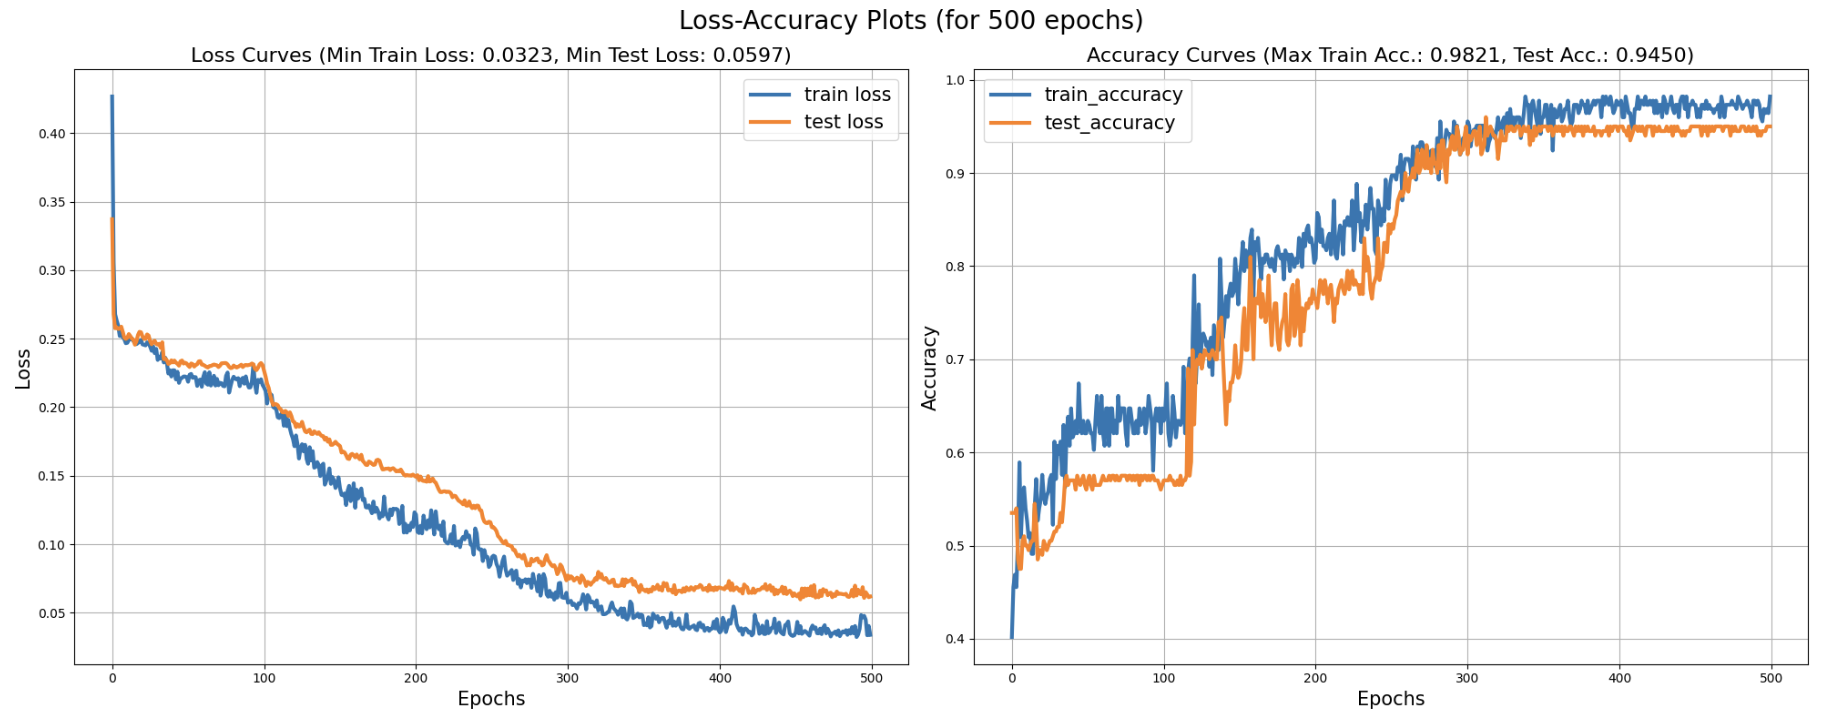
\includegraphics[width=0.7\textwidth]{plots/7_spiral_accloss.png}
%     \caption{Circular dataset (train, test set with 200 points each) after non-linear embedding}
% \end{figure}


We see that we are able to get accuracy of around 94\% on the swiss-roll test-data after adding non-linear features $x^2, x\times y, y^2$ for a MLP with only 2 hidden layers of 8 and 4 neurons each. This is a much bigger improvement over running the similar architecture on just the 2D data, without adding the non-linear features.

\begin{figure}[H]
    \centering
    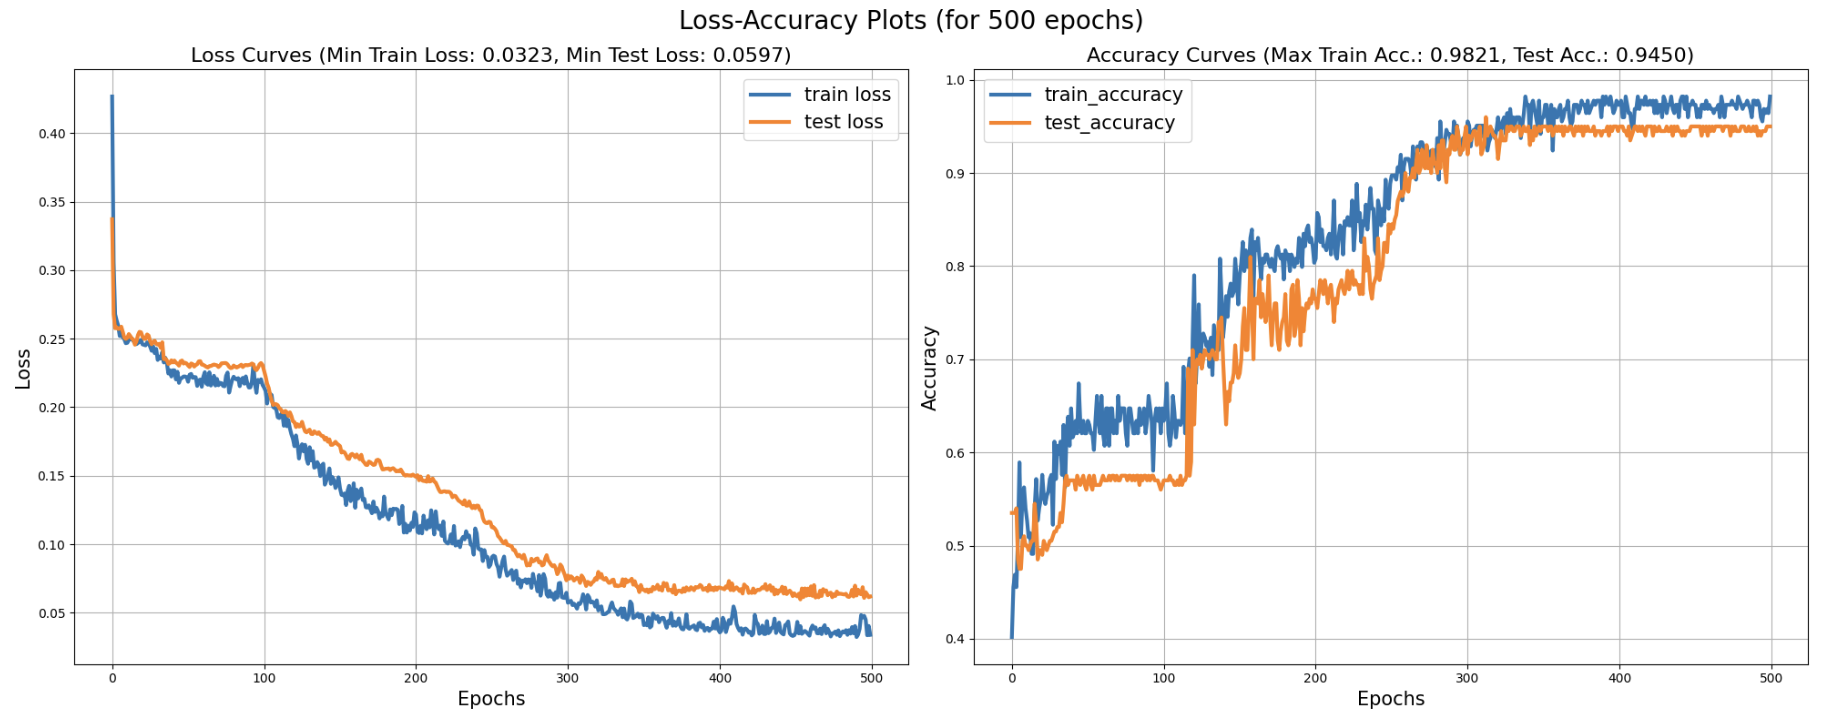
\includegraphics[width=0.8\textwidth]{plots/7_spiral_accloss.png}
    \caption{Loss Accuracy plot for swiss-roll data after adding $x^2, x\times y, y^2$ feature}

    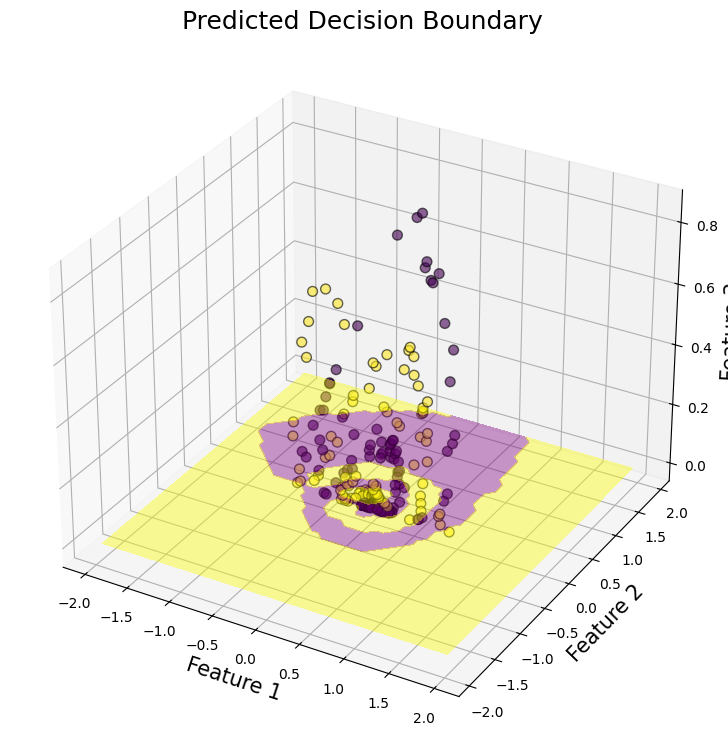
\includegraphics[width=0.7\textwidth]{plots/7_spiral_db.png}
    \caption{Predicted Decision boundary for swiss-roll data after adding $x^2 + y^2$ feature (x: feature 1, y: feature 2, $x\times y$: feature 3)}
\end{figure}

\end{solve}